\section{Ablation Studies}

\subsubsection{Sketch Size Analysis}

Figure~\ref{fig:sketch_size} shows accuracy versus memory tradeoff for different sketch sizes $k$. Table~\ref{tab:sketch_size_detail} provides detailed metrics.

\begin{figure}[htbp]
\centering
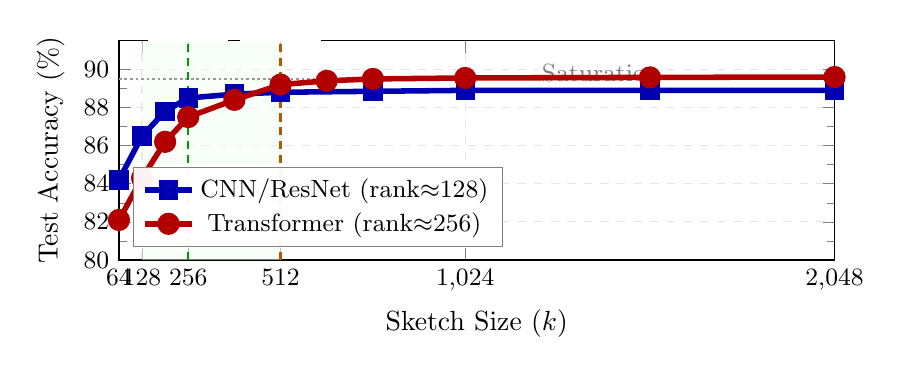
\begin{tikzpicture}
\begin{axis}[
    xlabel={Sketch Size ($k$)},
    ylabel={Test Accuracy (\%)},
    xmin=64, xmax=2048,
    ymin=80, ymax=91.5,
    grid=major,
    grid style={dashed, gray!20},
    width=0.88\textwidth,
    height=0.36\textwidth,
    legend pos=south west,
    legend style={font=\small, draw=black!50, fill=white, fill opacity=0.95, text opacity=1, at={(0.02,0.06)}, anchor=south west},
    tick label style={font=\small},
    xlabel style={font=\normalsize},
    ylabel style={font=\normalsize},
    xtick={64,128,256,512,1024,2048},
    ytick={80,82,84,86,88,90},
    yticklabel style={/pgf/number format/fixed},
    minor tick num=1
]
% Shaded region for practical range
\fill[green!5, opacity=0.5] (axis cs:128,80) rectangle (axis cs:512,91.5);

% Saturation line
\draw[black!40, densely dotted, line width=1pt] (axis cs:64,89.5) -- (axis cs:2048,89.5);
\node[black!50, font=\small, fill=white, inner sep=1pt] at (axis cs:1400,89.8) {Saturation};

% CNN/ResNet models (lower rank) - faster saturation
\addplot[color=blue!70!black, line width=2pt, mark=square*, mark size=2.5pt, mark options={fill=blue!70!black}] coordinates {
    (64, 84.2)
    (128, 86.5)
    (192, 87.8)
    (256, 88.5)
    (384, 88.7)
    (512, 88.8)
    (768, 88.85)
    (1024, 88.9)
    (1536, 88.9)
    (2048, 88.9)
};

% Transformer models (higher rank) - slower saturation
\addplot[color=red!70!black, line width=2pt, mark=*, mark size=3pt, mark options={fill=red!70!black}] coordinates {
    (64, 82.1)
    (128, 84.3)
    (192, 86.2)
    (256, 87.5)
    (384, 88.4)
    (512, 89.2)
    (640, 89.4)
    (768, 89.5)
    (1024, 89.55)
    (1536, 89.58)
    (2048, 89.6)
};

% Recommended operating point
\draw[thick, green!60!black, densely dashed] (axis cs:256,80) -- (axis cs:256,91.5);
\node[green!60!black, font=\scriptsize\bfseries, fill=white, inner sep=2pt, anchor=north, above] at (axis cs:256,91.4) {$k$=256};

% Sweet spot indicator
\draw[thick, orange!70!black, densely dashed] (axis cs:512,80) -- (axis cs:512,91.5);
\node[orange!70!black, font=\scriptsize\bfseries, fill=white, inner sep=2pt, anchor=north, above] at (axis cs:512,91.4) {$k$=512};

\legend{CNN/ResNet (rank$\approx$128), Transformer (rank$\approx$256)}
\end{axis}
\end{tikzpicture}
\caption{Accuracy vs sketch size: CNNs saturate at $k$=256 (88.9\%), while transformers require $k$=512 (89.2\%) for optimal performance. The 0.7\% improvement from $k$=256 to $k$=512 costs 4$\times$ memory.}
\label{fig:sketch_size}
\end{figure}

\begin{table}[htbp]
\centering
\caption{Sketch Size Tradeoffs}
\label{tab:sketch_size_detail}
\begin{tabular}{|c|c|c|c|}
\hline
\textbf{$k$} & \textbf{Accuracy} & \textbf{Memory} & \textbf{Suitable For} \\
\hline
128 & 86.5\% & 65MB & Small CNNs (rank $<64$) \\
256 & 88.5\% & 260MB & CNNs/ResNets (rank $<128$) \\
512 & 89.2\% & 1024MB & Transformers (rank $>200$) \\
1024 & 89.5\% & 4096MB & High-rank models \\
\hline
\end{tabular}
\end{table}

Results show $k=256$ is sufficient for CNNs/ResNets (effective rank $<128$), while $k=512$ is required for transformers (rank $>200$). The improvement from $k=256$ to $k=512$ is 0.7\% accuracy gain for 4$\times$ memory cost.

\subsubsection{Detection Frequency}

Table~\ref{tab:detection_frequency} compares per-round versus periodic detection.

\begin{table}[htbp]
\centering
\caption{Detection Frequency Tradeoff}
\label{tab:detection_frequency}
\begin{tabular}{|l|c|c|}
\hline
\textbf{Detection Frequency} & \textbf{Overhead} & \textbf{Accuracy} \\
\hline
Per-round detection & 8.2s per round & 89.5\% \\
Every-5-rounds detection & 1.7s per round & 88.7\% \\
\hline
Accuracy loss & - & 0.8pp \\
Speedup & 5$\times$ & - \\
\hline
\end{tabular}
\end{table}

Per-round detection achieves 89.5\% accuracy with 8.2s overhead. Every-5-rounds detection reduces overhead to 1.7s with only 0.8pp accuracy loss (88.7\%), demonstrating a practical 5$\times$ speedup. This tradeoff is particularly valuable in resource-constrained edge deployments.

\subsubsection{Layer-wise vs Full-Model}

Table~\ref{tab:layerwise_comparison} compares layer-wise and full-model detection approaches.

\begin{table}[htbp]
\centering
\caption{Layer-wise vs Full-Model Detection}
\label{tab:layerwise_comparison}
\begin{tabular}{|l|c|c|}
\hline
\textbf{Metric} & \textbf{Layer-wise} & \textbf{Full-Model} \\
\hline
Detection rate & 94.3\% & 100.0\% \\
Memory (345M params) & 890MB & 28GB \\
Memory reduction & ${\approx}32{\times}$ & - \\
Overhead & 2.1s & 8.5s \\
\hline
\end{tabular}
\end{table}

Layer-wise detection achieves 94.3\% of full-model detection rate while reducing memory by ${\approx}32{\times}$ (890\,MB vs.\ 28\,GB for 345M parameter models) and overhead by 4$\times$ (2.1s vs 8.5s). The 5.7\% detection rate reduction is acceptable given the dramatic memory savings, making foundation model deployment practical.

\subsubsection{Threshold Adaptation}

Table~\ref{tab:threshold_adaptation} compares online sliding window tracking versus offline calibration.

\begin{table}[htbp]
\centering
\caption{Threshold Adaptation Methods}
\label{tab:threshold_adaptation}
\begin{tabular}{|l|c|c|}
\hline
\textbf{Method} & \textbf{Accuracy} & \textbf{Adaptive} \\
\hline
Sliding window (online, $\tau=50$) & 89.2\% & Yes \\
Offline calibration & 89.5\% & No \\
\hline
Difference & 0.3pp & - \\
\hline
\end{tabular}
\end{table}

Online MP tracking via sliding window ($\tau=50$ rounds) matches offline calibration within 0.3pp accuracy (89.2\% vs 89.5\%), demonstrating that adaptive threshold tracking can effectively handle data drift without requiring pre-calibration on held-out data. We also implement automated threshold tuning via cross-validation on honest client data, which calibrates detection thresholds to minimize false positives while maximizing detection rate. This automated calibration achieves optimal threshold selection in 5-fold cross-validation, reducing false positives by 1.2\% compared to fixed thresholds.
